\documentclass{article}

%% Created with wxMaxima 12.01.0

\setlength{\parskip}{\medskipamount}
\setlength{\parindent}{0pt}
\usepackage[utf8]{inputenc}
\usepackage{graphicx}
\usepackage{color}
\usepackage{amsmath}

\definecolor{labelcolor}{RGB}{100,0,0}

\begin{document}

\noindent
%%%%%%%%%%%%%%%
%%% INPUT:
\begin{minipage}[t]{8ex}{\color{red}\bf
\begin{verbatim}
(%i1) 
\end{verbatim}}
\end{minipage}
\begin{minipage}[t]{\textwidth}{\color{blue}
\begin{verbatim}
w:2*%pi*50;
R:12;
L:22*10^-3;
z2:R^2+(w*L)^2;
Vm:230*sqrt(2);
E:180;
a:10*(%pi/180);
V(wt):=Vm*sin(wt+a);
C1:Vm/z2*(L*w*cos(a)-R*sin(a))+E/R,numer;
C2:Vm/z2*(R*sin(a)-L*w*cos(a)),numer;
C3:Vm/z2*(R*cos(a)+L*w*sin(a)),numer;
\end{verbatim}}
\end{minipage}
%%% OUTPUT:
\begin{math}\displaystyle
\parbox{8ex}{\color{labelcolor}(\%o1) }
100\,\pi 
\end{math}

\begin{math}\displaystyle
\parbox{8ex}{\color{labelcolor}(\%o2) }
12
\end{math}

\begin{math}\displaystyle
\parbox{8ex}{\color{labelcolor}(\%o3) }
\frac{11}{500}
\end{math}

\begin{math}\displaystyle
\parbox{8ex}{\color{labelcolor}(\%o4) }
\frac{121\,{\pi }^{2}}{25}+144
\end{math}

\begin{math}\displaystyle
\parbox{8ex}{\color{labelcolor}(\%o5) }
115\,{2}^{\frac{3}{2}}
\end{math}

\begin{math}\displaystyle
\parbox{8ex}{\color{labelcolor}(\%o6) }
180
\end{math}

\begin{math}\displaystyle
\parbox{8ex}{\color{labelcolor}(\%o7) }
\frac{\pi }{18}
\end{math}

\begin{math}\displaystyle
\parbox{8ex}{\color{labelcolor}(\%o8) }
\mathrm{V}\left( wt\right) :=Vm\,\mathrm{sin}\left( wt+a\right) 
\end{math}

\begin{math}\displaystyle
\parbox{8ex}{\color{labelcolor}(\%o9) }
23.01045703879069
\end{math}

\begin{math}\displaystyle
\parbox{8ex}{\color{labelcolor}(\%o10) }
-8.01045703879069
\end{math}

\begin{math}\displaystyle
\parbox{8ex}{\color{labelcolor}(\%o11) }
22.08027049835779
\end{math}
%%%%%%%%%%%%%%%


\noindent
%%%%%%%%%%%%%%%
%%% INPUT:
\begin{minipage}[t]{8ex}{\color{red}\bf
\begin{verbatim}
(%i12) 
\end{verbatim}}
\end{minipage}
\begin{minipage}[t]{\textwidth}{\color{blue}
\begin{verbatim}
i(wt):=C1*%e^(-R/(L*w)*wt)+C2*cos(wt)+C3*sin(wt)-(E/R);
wxplot2d([i(wt)],[wt,-0.01,6],[y,-40,10],[gnuplot_preamble, "set grid"]);
\end{verbatim}}
\end{minipage}
%%% OUTPUT:
\begin{math}\displaystyle
\parbox{8ex}{\color{labelcolor}(\%o12) }
\mathrm{i}\left( wt\right) :=C1\,{e}^{\frac{-R}{L\,w}\,wt}+C2\,\mathrm{cos}\left( wt\right) +C3\,\mathrm{sin}\left( wt\right) -\frac{E}{R}
\end{math}

\begin{math}\displaystyle
\parbox{8ex}{\color{labelcolor}(\%t13) }
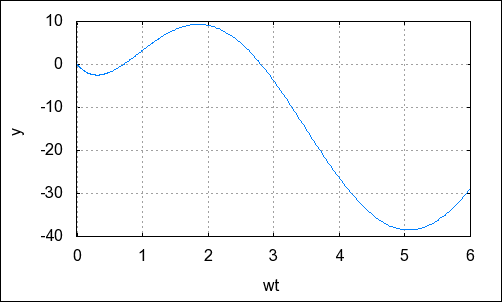
\includegraphics[width=9cm]{problema_3_img/problema_3_1.png}
\end{math}

\begin{math}\displaystyle
\parbox{8ex}{\color{labelcolor}(\%o13) }

\end{math}
%%%%%%%%%%%%%%%


\noindent
%%%%%%%%%%%%%%%
%%% INPUT:
\begin{minipage}[t]{8ex}{\color{red}\bf
\begin{verbatim}
(%i14) 
\end{verbatim}}
\end{minipage}
\begin{minipage}[t]{\textwidth}{\color{blue}
\begin{verbatim}
kill(all);
\end{verbatim}}
\end{minipage}
%%% OUTPUT:
\begin{math}\displaystyle
\parbox{8ex}{\color{labelcolor}(\%o0) }
done
\end{math}
%%%%%%%%%%%%%%%

\end{document}
